En esta práctica se calcula la cinemática directa para manipuladores tridimensionales. 
Se modifica la morfología del robot indicando la longitud de los elementos rígidos, así como la existencia de articulaciones de revolución o prismáticas.
Al ejecutar el script se indican los valores de las variables articulares.

\section{Código Implementado}
\subsection{Análisis}
El script proporcionado contiene todo el código necesario para calcular la cinemática directa y visualizar los manipuladores. 
Solamente se deben modificar ciertos parámetros para adaptar el script a la morfología del robot:
\begin{itemize}
   \item \texttt{nvar} Número de variables que se introduciran al ejecutar el programa, correspondientes a las variables articulares.
   \item \texttt{Parámetros de Denavit–Hartenberg} son 4 vectores, uno para cada parámetro. El tamaño del vector se corresponde al número de articulaciones.
   \item \texttt{Orígenes para cada articulación} un vector con las coordenadas homogéneas de cada articulación.
   \item \texttt{Matrices T} son matrices que permiten realizar la transformación de un sistema de coordenadas a otro.
   Las matrices entre sistemas consecutivos son triviales, y se construyen con sus parámetros de Denavit–Hartenberg.
   Las matrices que describen la transformación entre sistemas no consecutivos se obtienen multiplicando las matrices de transformación de los sistemas intermedios.
   Por ejemplo, la matriz T02, que transforma el sistema de coordenadas 0 al 2, se obtiene realizando el producto de las matrices T01 y T12.
   \item \texttt{Coordenadas de cada articulación} se calcula el origen de coordenadas del sistema de cada articulación mediante el producto de la matriz de transformación T0X y el origen de coordenadas oXX.
   \item \texttt{Visualización del robot} se deben modificar las instrucciones de visualización para adaptarlas a la morfología del robot, incluyendo los origenes de coordenadas calculados que se quieren visualizar.
\end{itemize}

En la figura~\ref{chapter:intro2} se muestra el fragmento del script que se debe modificar.
\begin{figure}[htb]
   \centering
   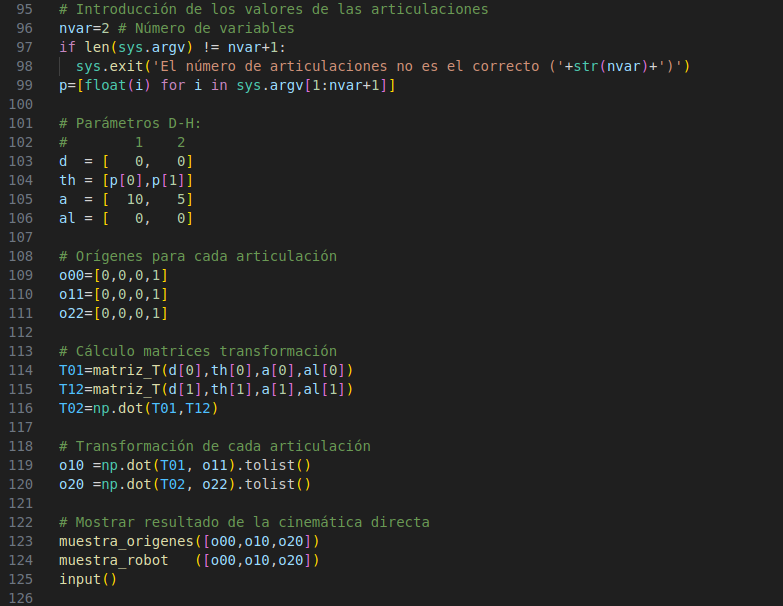
\includegraphics[width=1\linewidth]{images/cin_dir_1.png}
   \caption{Porción del código que se debe modificar para cada manipulador}
   \label{chapter:intro2}
\end{figure}

\bigskip Al ejecutar el código se deben proporcionar como parámetros los valores de las variables articulares: unidades de longitud en el caso de las articulaciones prismáticas, y grados de rotación en el caso de las articulaciones de revolución. 

\subsection{Complejidad}
La complejidad del código depende del número de articulaciones del manipulador. Por cada nueva articulación, solamente es necesario realizar dos productos de matrices de transformación homogénea. Uno para obtener la matriz de transformación y otro para obtener las coordenadas de la articulación. Por tanto, la complejidad es lineal respecto al número de articulaciones.
%%%%%%%%%%%%%%%%%%%%%%%%%%%%%%%%%%%%%%%%%%%%%%%%%%%%%%%%%%%%%
\section{Ejemplo}
Se emplea el Manipulador 3 de entre los propuestos para visualizar la cinemática directa. Se ha elegido puesto que tiene suficiente complejidad para ilustrar correctamente la práctica, pero sin ser excesiva.
\begin{figure}[htb]
   \centering
   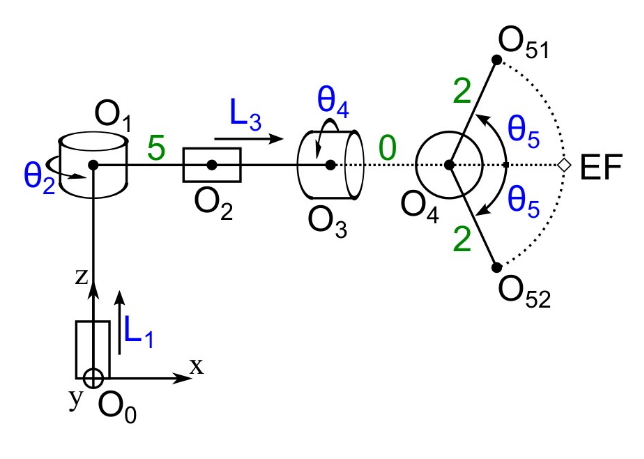
\includegraphics[width=0.6\linewidth]{images/cin_dir_2.png}
   \caption{Manipulador 3}
   \label{chapter:manipulador3}
\end{figure}

\subsection{Código}
La figura \ref{chapter:codigo2} muestra el código modificado para el manipulador 3.
Cabe destacar que se necesita emplear un sistema de coordenadas auxiliar entre O1 y O2 para que el sitema sea dextrógiro y compatible Denavit-Hartenberg.
También resulta reseñable que para la visualización del manipulador, en las 2 funciones pertinentes, los puntos O51 y O52 se agrupan en un mismo vector, para señalar que son 2 bifurcaciones desde el punto anterior. 
\begin{figure}[htb]
   \centering
   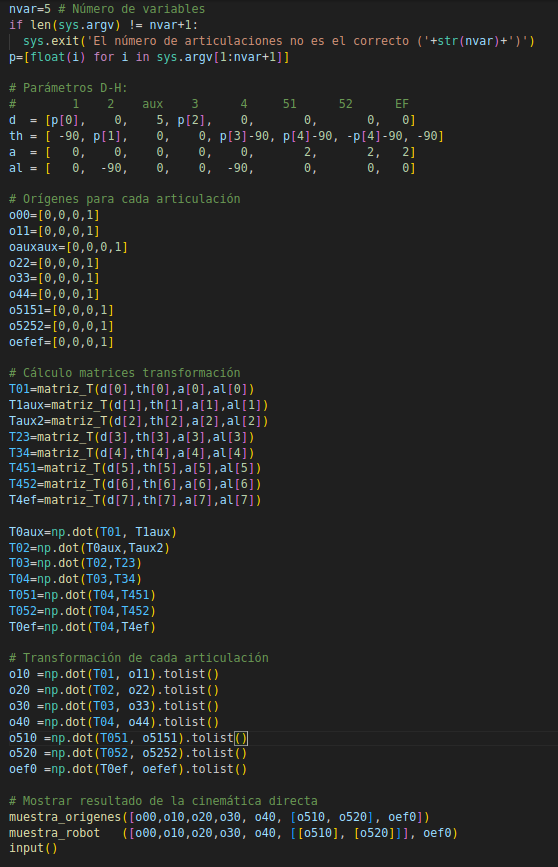
\includegraphics[width=0.8\linewidth]{images/cin_dir_3.png}
   \caption{Código para el manipulador 3}
   \label{chapter:codigo2}
\end{figure}

\subsection{Ejecución}
En primer lugar, en la figura \ref{chapter:ejecucion1} se muestra un ejemplo de ejecución con todas las variables articulares a 0. Observamos que algunos orígenes se solapan, por ejemplo O0 y O1, o O51 y O52.
\begin{figure}[htb]
   \centering
   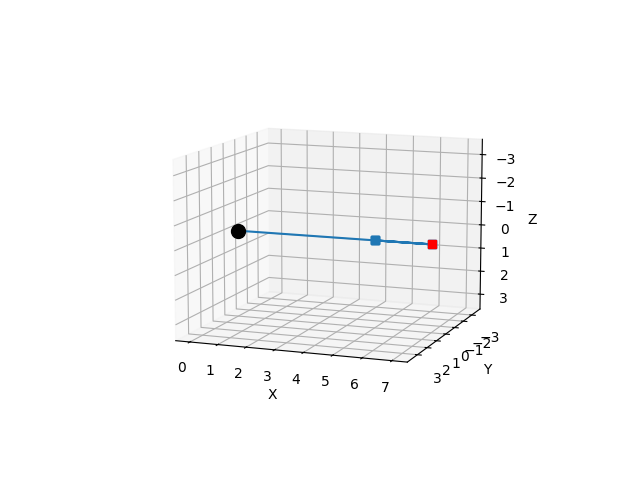
\includegraphics[width=0.8\linewidth]{images/cin_dir_4.png}
   \caption{Ejecución 1}
   \label{chapter:ejecucion1}
\end{figure}

A continuación, probamos dando valor de 5 a las articulaciones prismáticas y 30º para la articulación O4. Dejamos el resto a 0. De esta forma, como observamos en la figura \ref{chapter:ejecucion2a} el manipulador se asemeja al diagrama del ejercicio.
\begin{figure}[htb]
   \centering
   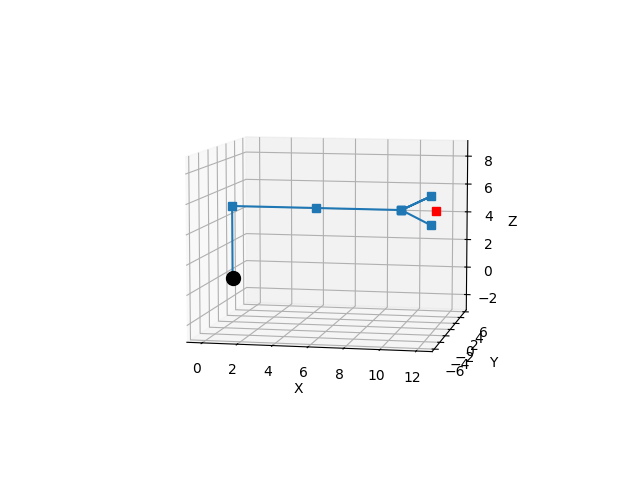
\includegraphics[width=0.8\linewidth]{images/cin_dir_5.png}
   \caption{Ejecución 2}
   \label{chapter:ejecucion2a}
\end{figure}
\begin{figure}[htb]
   \centering
   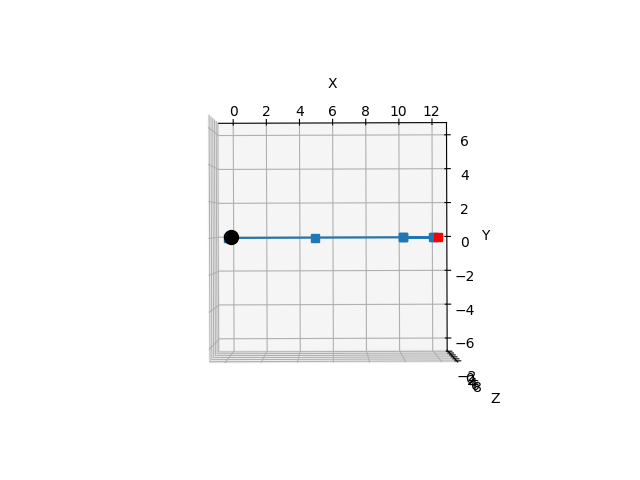
\includegraphics[width=0.8\linewidth]{images/cin_dir_6.png}
   \caption{Ejecución 2, perspectiva vertial}
   \label{chapter:ejecucion2b}
\end{figure}

En último lugar, aplicamos una rotación de 30º en las articulaciones O1 y O3. Observamos el resultado en la figura \ref{chapter:ejecucion3a}.
\begin{figure}[htb]
   \centering
   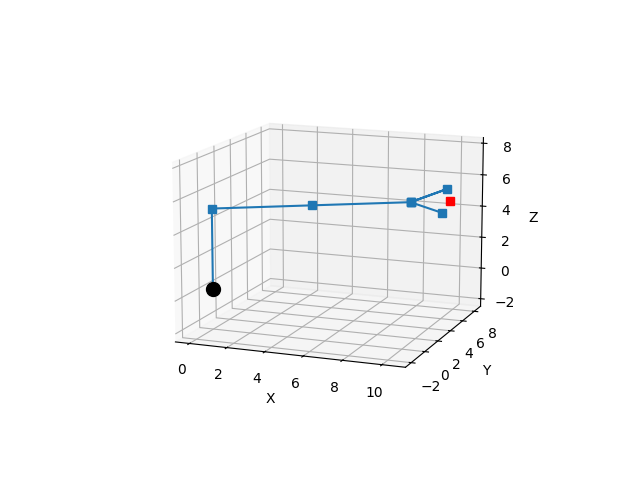
\includegraphics[width=0.8\linewidth]{images/cin_dir_7.png}
   \caption{Ejecución 3}
   \label{chapter:ejecucion3a}
\end{figure}
\begin{figure}[htb]
   \centering
   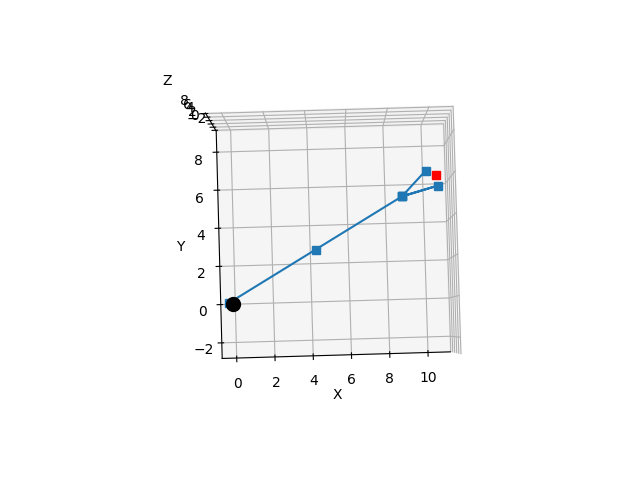
\includegraphics[width=0.8\linewidth]{images/cin_dir_8.png}
   \caption{Ejecución 3, perspectiva vertial}
   \label{chapter:ejecucion3b}
\end{figure}

De esta forma, hemos comprobado que el código funciona correctamente y que la descripción del manipulador realizada es correcta.

\section{Mejoras}
En esta práctica no se han implementado mejoras, pero se proponen algunas que podrían ser interesantes.
\begin{itemize}
   \item \texttt{Lectura de JSON} se podría implementar la lectura de la morfología del robot desde un ficheor JSON, evitando tener que modificar el script para cada manipulador.
   \item \texttt{Modificación de los parámetros en tiempo real} Sería de gran utilidad poder modificar las variables articulares mientras se visualiza el manipulador, para poder estudiar fácilmente cómo lo afectan.
\end{itemize}

\section{Conclusions}
We have studied the forward kinematics of a 3D manipulator. We have seen that we can characterize any manipulator by its Denavit-Hartenberg parameters, and that it is easy and fast to calculate the coordinates of each joint. 
We have also seen that the visualization of the manipulator is very useful to understand its behavior and to check that the calculations made to obtain the parameters are correct.

\bigskip Although the script provided is very useful, it has room for improvements. Also, we still have to manually calculate the Denavit-Hartenberg parameters, which can be a tedious task for complex manipulators.